\documentclass[tikz,border=10pt]{standalone}
\usepackage{tikz}
\usepackage{pgfplots}
\usetikzlibrary{patterns, arrows.meta}

\begin{document}
\sffamily
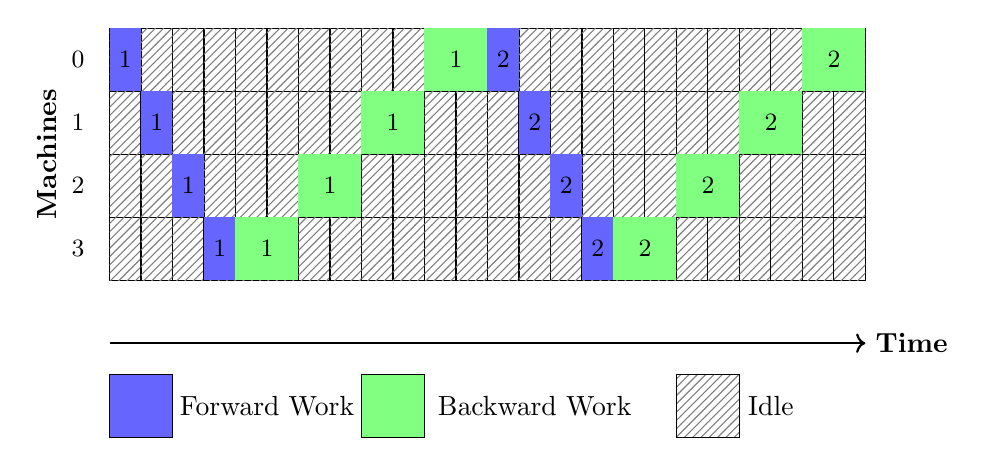
\begin{tikzpicture}

% Define styles
\tikzstyle{forward}=[fill=blue!60]
\tikzstyle{backward}=[fill=green!50]
\tikzstyle{idle}=[pattern=north east lines, pattern color=black!50]
\tikzstyle{label}=[font=\small]

% Parameters
\def\rows{4}
\def\cols{24}
\def\cellsize{0.8}

\pgfmathsetmacro{\rowsm}{\rows - 1}
\pgfmathsetmacro{\colsm}{\cols - 1}

% Draw grid and idle cells
\foreach \r in {0,...,{\rowsm}} {
  \foreach \c in {0,...,{\colsm}} {
    \draw[black] (0.5*\c*\cellsize,-\r*\cellsize) rectangle ++(0.5*\cellsize,\cellsize);
    \fill[idle] (0.5*\c*\cellsize,-\r*\cellsize) rectangle ++(0.5*\cellsize,\cellsize);
  }
}

% Fill Forward and Backward Work
% Format: \fill[style] (col,row) rectangle ++(1,1); \node at (col,row) {text};

% Forward Work (blue)
\foreach \x/\y/\text in {0/0/1, 1/1/1, 2/2/1, 3/3/1, 12/0/2, 13/1/2, 14/2/2, 15/3/2} {
  \fill[forward] (\x*0.5*\cellsize,-\y*\cellsize) rectangle ++(\cellsize*0.5,\cellsize);
  \node[label] at (\x*0.5*\cellsize+0.25*\cellsize,-\y*\cellsize+0.5*\cellsize) {\text};
}

% Backward Work (green)
\foreach \x/\y/\text in {2/3/1, 3/2/1, 4/1/1, 5/0/1, 8/3/2, 9/2/2, 10/1/2, 11/0/2} {
  \fill[backward] (\x*\cellsize,-\y*\cellsize) rectangle ++(\cellsize,\cellsize);
  \node[label] at (\x*\cellsize+0.5*\cellsize,-\y*\cellsize+0.5*\cellsize) {\text};
}

% Machine labels
\foreach \r [evaluate=\r as \m using int(\r)] in {0,...,\rowsm} {
  \node[label] at (-0.5*\cellsize,-\r*\cellsize+0.5*\cellsize) {\m};
}
\node[rotate=90] at (-1*\cellsize,-1*\cellsize) {\textbf{Machines}};

% Time axis
\draw[thick, ->] (0,-4*\cellsize) -- (12*\cellsize,-4*\cellsize) node[anchor=west] {\textbf{Time}};

% Legend
\begin{scope}[shift={(0,-5.5*\cellsize)}]
  \draw[forward] (0,0) rectangle ++(\cellsize,\cellsize);
  \node at (2.5*\cellsize,0.5*\cellsize) {Forward Work};

  \draw[backward] (4*\cellsize,0) rectangle ++(\cellsize,\cellsize);
  \node at (6.75*\cellsize,0.5*\cellsize) {Backward Work};

  \draw[pattern=north east lines, pattern color=black!50] (9*\cellsize,0) rectangle ++(\cellsize,\cellsize);
  \node at (10.5*\cellsize,0.5*\cellsize) {Idle};
\end{scope}

\end{tikzpicture}
\end{document}
